% -----------
% Copyright 2013-2014, Andrew Lindesay
% Distributed under the terms of the MIT License.
% -----------

\section{Deployment}

This section outlines the approximate steps to deploy the web application-server.  The application-server build process produces a  `stand-alone' java program.  This build artifact is a packaged `jar' file that contains the \href{http://tomcat.apache.org}{Tomcat} servlet container as well as the web application.  Upon launching, it will unbundle necessary parts and start-up listening on a socket for inbound HTTP requests.

\fcolorbox{red}{white}{\parbox{\textwidth}{\color{red} The default database installs a user with the nickname of `root' with a known password of `p4mphl3t'.  This password {\bf must} be changed before the system is made available over a network.}}

\fcolorbox{red}{white}{\parbox{\textwidth}{\color{red}The API-related HTTP traffic into the application server uses basic or token bearer authentication.  Either technique exposes authentication details in the request and response.  For this reason it is advised that HTTP traffic to and from the application server be transported as secure HTTP (https) in order to prevent a third party from reading the HTTP headers and extracting this information.}}

Please see \ref{prerequisites} for prerequisites required for running this software and \ref{buildandrelease} for information about obtaining a build product and possibly also creating a release version.  The build product that you will require for deployment can be found at;

\framebox{\tt haikudepotserver-webapp/target/haikudepotserver-webapp-1.2.3-war-exec.jar}

The leaf-name will vary depending on the release that is being build.  You should also refer to \ref{config} for details of the format and keys for the configuration file.  You will need to create a configuration file for your deployment.

To launch the binary with 256 megabytes of heap memory, issue a command similar to;

\begin{verbatim}
java \
 -Xmx512m \
 -Dfile.encoding=UTF-8 \
 -Duser.timezone=GMT0 \
 -Djava.awt.headless=true \
 -Dconfig.properties=file:///etc/haikudepotserver/config.properties \
 -jar haikudepotserver-webapp-1.2.3-war-exec.jar \
 -resetExtract \
 -extractDirectory /var/cache/haikudepotserver
\end{verbatim}

By default the logging will be streamed to stdout/stderr.  It is possible to configure this using a \href{http://logback.qos.ch/}{logback} logging configuration file.

There are a handful of other easily-accessed command line options which can be used to fine-tune the deployment.  These can be viewed by executing the binary as follows;

\begin{verbatim}
java \
 -jar haikudepotserver-webapp-1.2.3-war-exec.jar \
 -h
\end{verbatim}

\subsection{Setting Up Repositories}
\label{settinguprepositories}

The application server will pull ``.hpkr'' files from remote repositories that contain information about the packages at that repository.  Authenticated as root, it is possible to use the ``more'' link at the top of the home page to get to the repositories, to add a repository and to trigger the import of a repository.  There also exists an HTTP GET invocation (see \ref{api-importrepositorydata}) that can be made to trigger the import of a repository from another system\footnote{Such as the HPKR assembly process}.

\subsection{Maintenance Tasks}

Some maintenance tasks are scheduled.  These tasks are scheduled from outside the application server in order to simplify a multi-instance deployment topology.  A simple approach to this is to schedule using the cron tool.  This would require a ``crontab'' entry such as;

 \framebox{\tt 14 * * * * curl "http://localhost:8080/maintenance/mediumterm"}

 The host and port should be adjusted to suit your deployment environment.

\subsection{Accessing the Web Environment}

Once running, the web environment will be accessible from;

\framebox{\tt http://localhost:8080/}

\subsection{Deployment with RPM}

The build system, when executed on a linux host, will produce RPMs that can be deployed into an RPM-based linux system.  The RPMs do not have any dependencies and so both java and Postgres database server will need to be installed before the application server can be successfully started --- see \ref{prerequisites}.  Two RPMs are built;

\begin{tabular}{|l|l|l|}
\hline
Variant & Project & HTTP Port \\
\hline
Production & {\tt haikudepotserver-rpm-production} & 8801 \\
Test & {\tt haikudepotserver-rpm-test} & 8701 \\
\hline
\end{tabular}

The production variant has names and paths that are simply ``{\tt haikudepotserver}'' whereas the test variant has names and paths that are of the form ``{\tt haikudepotserver-test}''.  In the instructions that follow, the test variant has been indicated by a colored suffix ``{\tt\color{magenta} -test}''.

The RPM is built with the ``package'' maven goal.  The RPM build product can be found at this path from that module;

\framebox{\tt ../target/rpm/haikudepotserver{\color{magenta} -test}/RPMS/noarch/}

\subsubsection{Installing}

The RPM can be installed with the following command making an obvious reference to the RPM file.

\framebox{\tt rpm -ivh haikudepotserver{\color{magenta} -test}-1.0.2.rpm}

The RPM can be uninstalled with the following command;

\framebox{\tt rpm -e haikudepotserver{\color{magenta} -test}}

It would be prudent to first ensure that the application server is not running before uninstalling it.

\subsubsection{File Locations}

The RPM will install files into the following locations;

\begin{tabular}{|l|l|}
\hline
Location & Description \\
\hline
{\tt /var/log/haikudepotserver{\color{magenta} -test}/..} & Log files from the application server \\
{\tt /opt/haikudepotserver{\color{magenta} -test}/..} & Application server binary resources \\
{\tt /var/cache/haikudepotserver{\color{magenta} -test}/..} & Operational files for the application server \\
{\tt /etc/haikudepotserver{\color{magenta} -test}/..} & Configuration files \\
{\tt /etc/logrotate.d/..} & Log rotation configuration \\
{\tt /etc/init.d/haikudepotserver{\color{magenta} -test}} & Start and stop script \\
\hline
\end{tabular}

\subsubsection{Start and Stop}

The installed application server can be started with the following command, referencing the RPM file;

\framebox{\tt service haikudepotserver{\color{magenta} -test} start}

The installed application server can be stopped with the following command;

\framebox{\tt service haikudepotserver{\color{magenta} -test} stop}

\subsubsection{Automatic Startup and Shutdown}

The installed application server can be configured to startup automatically using the following command;

\framebox{\tt chkconfig --add haikudepotserver{\color{magenta} -test}}

The installed application can later be prevented from automatic startup using the following command;

\framebox{\tt chkconfig --del haikudepotserver{\color{magenta} -test}}

\subsubsection{RPM Assembly / Maven}

\begin{figure}
\centering
\vspace{.2in}
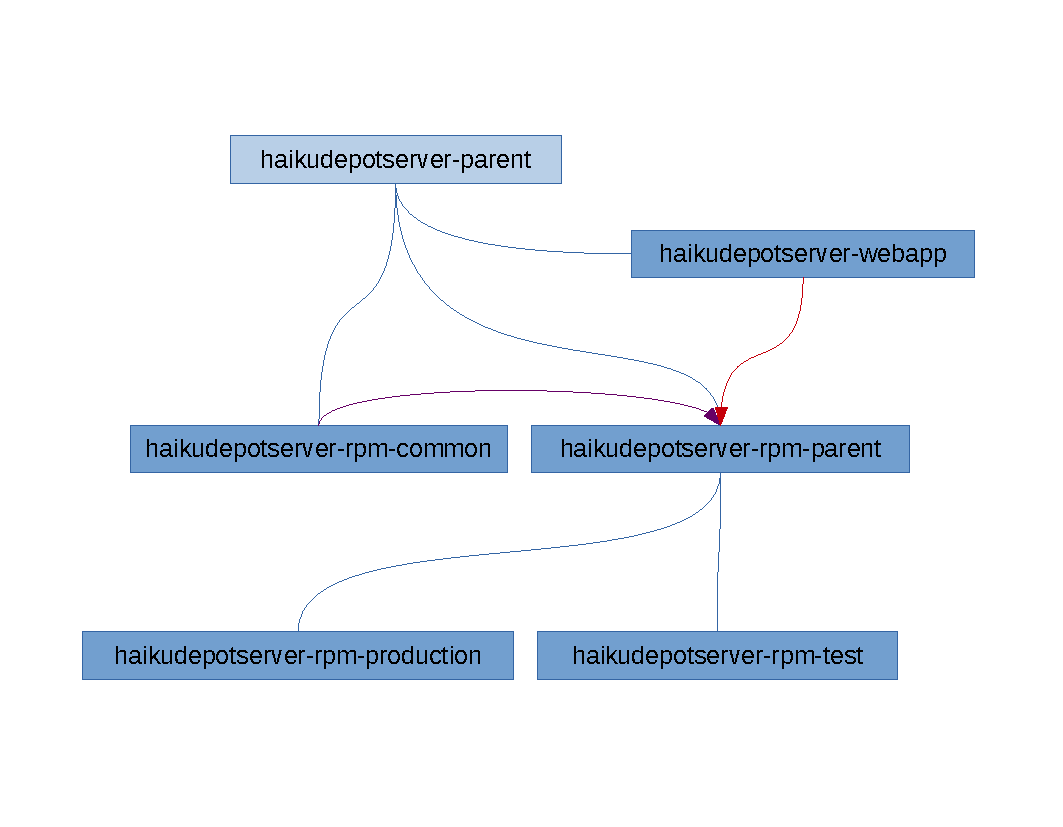
\includegraphics[width=6.5in]{img-rpm-package-assembly-diagram.pdf}
\caption{The maven modules that are related to the RPM assembly process and how they inter-relate.}
\label{\thefigure}
\end{figure}

There are a number of inter-related maven modules that work together to generate the RPMs.  These are shown in figure {\thefigure}.  The blue lines show module inheritance.  An ``reactor POM'' (not shown here) will prevent the RPM from being assembled unless the build system is on a linux host.  It does this by using a maven profile that is triggered by the operating system type.

The module {\tt haikudepotserver-rpm-common} provides (purple line) resources for the RPM assembly that are common to the variants (production and test).  This means that the same resources will assemble both variants.  Note that the resources are intended to be {\it filtered} in the RPM assembly process so they contain token-replacement strings such as {\tt \$\{rpm.variant\}}.  The filtering occurs late in the RPM assembly process.  These resources are unpacked in both of the RPM assembly modules {\tt haikudepotserver-rpm-production} and {\tt haikudepotserver-rpm-test}.

Both of the RPM assembly modules have {\tt haikudepotserver-rpm-parent} as a parent and this parent has the configuration (using a maven plugin called {\tt rpm-maven-plugin}) for the assembly so that the configuration of the assembly is shared between the two assembly modules.  The {\tt haikudepotserver-rpm-parent} also introduces a dependency (red line) on the {\tt haikudepotserver-webapp} module in order that the web application build-product can be included in the RPMs.